\documentclass[sigconf,screen,review,natbib]{acmart}
\AtBeginDocument{%
\providecommand\BibTeX{{%
\normalfont B\kern-0.5em{\scshape i\kern-0.25em b}\kern-0.8em\TeX}}}

\setcopyright{acmcopyright}
\copyrightyear{2023}
\acmYear{2023}
\acmDOI{XXXXXXX.XXXXXXX}

\acmConference[PPDP '23]{25th International Symposium on
	Principles and Practice of Declarative Programming}{October 22--23,
	2023}{Cascais, Lisbon, Portugal}

\usepackage{microtype}
\usepackage{tikz,tikz-qtree}
\usetikzlibrary{positioning}
\usetikzlibrary{arrows.meta, shapes.misc, positioning}
\usepackage{subfig}
\theoremstyle{definition}
\newtheorem{exmp}{Example}[section]
\usepackage[ruled, vlined, linesnumbered]{algorithm2e}
\SetKw{True}{true}
\SetKw{False}{false}
\SetKwData{typeInt}{Int}
\SetKwData{typeRat}{Rat}
\SetKwData{Defined}{Defined}
\SetKwFunction{parseStatement}{parseStatement}
\usepackage{libertine}

\title{A Differential Datalog Interpreter}

\author{Bruno Rucy Carneiro Alves de Lima}
\orcid{1234-5678-9012}
\affiliation{%
	\institution{University of Tartu}
	\department{Institute of Computer Science}
	\city{Tartu}
	\country{Estonia}
}
\email{bruno98@ut.ee}

\author{Merlin Kramer}
\affiliation{%
	\institution{unaffiliated}
	\city{Wuppertal}
	\country{Germany}
}
\email{merlin.kramer@gmail.com}

\author{Kalmer Apinis}
\affiliation{%
	\institution{University of Tartu}
	\department{Institute of Computer Science}
	\city{Tartu}
	\country{Estonia}
}
\email{kalmera@ut.ee}

\begin{abstract}
	The core reasoning task for datalog engines is materialization, the evaluation of a datalog program over
	a database alongside its physical incorporation into the database itself. The de-facto method of computing
	it, is through the recursive application of inference rules. Due to it being a costly operation, it is a must
	for datalog engines to provide incremental materialization, that is, to adjust the computation to new
	data, instead of restarting from scratch. One of the major caveats, is that deleting data is notoriously more
	involved than adding, since one has to take into account all possible data that has been entailed from what
	is being deleted. Differential Dataflow is a computational model that provides efficient incremental
	maintenance, notoriously with equal performance between additions and deletions, and work distribution, of
	iterative dataflows. In this paper we investigate the performance of materialization with three reference
	datalog implementations, out of which one is built on top of a lightweight relational engine, and the two others
	are differential-dataflow and non-differential versions of the same rewrite algorithm, with the same optimizations.
\end{abstract}

\keywords{datalog, incremental view maintenance, differential dataflow}

\begin{document}

\maketitle

\section{Introduction}
Datalog\cite{datalog}, the canonical language for reasoning over relational databases, ground fact stores, is a
declarative language used to evaluate sets of possibly-recursive restricted horn clauses, programs, while
remaining not Turing complete. Evaluating a program entails computing implicit consequences over a fact
store, yielding new facts.

Materialization, or the physical storage of a program's consequences, eliminates the need for reasoning
during query answering. Maintaining this computation is essential for modern Datalog use-cases, as it
relates to the broader problem of incremental view maintenance.

While the semi-naive evaluation method\cite{datalog} efficiently handles additions, deletions are often less efficient, as
retracting a fact may naively imply deleting all data derived from it. The delete-rederive\cite{dred} method addresses
this issue by computing the materialization adjustment through the generation of new Datalog programs, first
calculating all possible deletions, and then determining alternative derivations. The difference between these
sets represents the actual facts to be deleted.

However, using two distinct algorithms for additions and deletions results in different performance characteristics,
potentially causing severe biases. For example, when a large portion of ground facts are deleted, delete-rederive
could be significantly more expensive than re-materializing.

A promising way to tackle incremental maintenance in a more uniform manner is to use differential dataflow, a
programming model that efficiently processes and maintains large-scale possibly recursive dataflow computations. Central
to it is the notion of fine-grained tracking, with partially-ordered timestamps, and processing differences between
collections of data, rather than entire collections themselves. This approach facilitates efficient updates in response
to changes in the underlying data\cite{differential_dataflow}.

In the context of datalog, differential dataflow presents an opportunity to address the performance challenges
arising from handling additions and deletions. Contrary to traditional methods, such as semi-naive evaluation for
additions and delete-rederive for deletions, differential dataflow provides a unified and efficient approach to
incremental view maintenance.

The utilization of partially ordered timestamps and arrangements allows differential dataflow to precisely
identify affected parts of the computation and to recompute only the necessary components. This leads to
a more efficient handling of incremental updates in Datalog evaluation, as the system can focus on affected
sub-computations rather than re-evaluating the entire program. Furthermore, there also is first-class support
for both automatic parallelism and distributed computing, contributing to enhanced performance and scalability.

DDLog\cite{ddlog} has been the only attempt at building a datalog engine that utilized differential dataflow.
Similarly to the high-profile reasoner Souffle\cite{souffle}, it is a compiler, in which a datalog program
becomes an executable low-level language program, C++ in Souffle's case, and Rust for DDLog. The rationale for
the language choice, is that differential dataflow's canonical implementation lives as a heavily optimized
map-reduce-like framework written in Rust.

Notably, given that DDLog is a compiler, it is not suited for situations where either the program is expected
to be dynamic, with rules being added or removed, or where new programs ought to be evaluated during run
time, therefore restricting its use case to the specific scenarios where such drawbacks are acceptable.

There has been no study evaluating the isolated benefit of differential dataflow to datalog evaluation. Therefore
the suitability of differential dataflow in this context remains unclear, emphasizing the importance of further
research on its potential benefits and limitations in incremental view maintenance.
\paragraph{Contributions.} In this work, we directly address the posited research question by developing a datalog
interpreter utilizing differential dataflow. We then compare our implementation with other prototypical datalog
interpreters, created from scratch, that share as many components as it is reasonable, in order to isolate
the effect of differential dataflow in both runtime performance and memory efficiency. This allows us to more
accurately empirically assess how does differential dataflow in itself fare against more traditional approaches.

Unlike DDLog, which compiles a datalog program into its evaluation as a fixed differential dataflow program, our
approach involves writing a single differential dataflow program capable of evaluating any datalog program. This
eliminates the need for compilation and provides the additional benefit of incremental maintenance for both rule
removals and additions.
\paragraph{Structure of the paper.}
\begin{itemize}
	\item{\textbf{Background.}} A brief recapitulation of the general background, with datalog, its evaluation
	methods, and the delete-rederive method being formally introduced.
	\item{\textbf{Differential Evaluation.}} Differential Dataflow, and the translation of datalog evaluation to
	a dataflow is showcased and explained.
	\item{\textbf{System.}} The developed interpreters are described, alongside with all optimizations and
	benchmark-relevant information.
	\item{\textbf{Benchmarks.}} An empirical evaluation of all reasoners, over multiple different programs and
	datasets is undertaken.
\end{itemize}
\section{Related Work}

\textbf{Differential Dataflow Applications.} There are two relevant differential dataflow projects that are worth
mentioning. One of them is Graspan, a parallel graph processing system that uses differential dataflow for efficient
incremental computation of static program analyses over large codebases.

Graspan models the program analysis problem as a reachability problem on a graph, where nodes represent program elements
and edges represent the relationships between these elements. It leverages differential dataflow to incrementally update
the analysis results in response to changes in the input graph, which can be due to code modifications or updates to
the analysis rules. Graspan has demonstrated its ability to scale to large codebases and provide low-latency updates
for various static analyses, including points-to analysis, control-flow analysis, and data-flow analysis.

Another project of interest is DBSP\cite{dbsp}, a recent development, that started from the need for a more concise
theoretical definition of differential dataflow. All of DBSP operators are based on differential dataflow's, however, its
computational model is less powerful as it does not allow updates to past values in a stream, and it is also assumed that
inputs arrive in time order. DBSP can express both incremental and non-incremental computations, with the former not being
possible in differential dataflow.

\textbf{Datalog engines.} There are two kinds of datalog engines. The first encompasses those that compile
a datalog program to usually a systems-level programming language, and the second are interpreters, able to
evaluate any datalog program.

Soufflé is a prominent example of a datalog compiler that translates datalog programs into high-performance
C++ code. It incorporates several optimization techniques, such as parallel execution with highly specialized data
structures\cite{souffle_btree}, and nearly optimal join ordering\cite{souffle_join}. Notably, its development has
been an unparalleled source of articles on the engineering of reasoners.

DDLog As previously mentioned, compiles datalog to differential dataflow, achieving efficient differential data updates
for datalog programs. It demonstrates the applicability of differential dataflow in the context of declarative logic
programming and incremental view maintenance.

The majority of reasoners recently developed have been mostly interpreters, further split into distributed or
shared memory systems. Out of the shared memory ones, the most notable are RDFox\cite{rdfox}, a highly specialized
and performant reasoner that is tailored to the semantic web needs, RecStep\cite{recstep}, that builds on top of a
highly efficient relational engine, and DCDatalog\cite{dcdatalog}, that builds upon the query optimizer DeALS\cite{deals}
and extends a work that establishes how some linear datalog programs could be evaluated in a lock-free manner, to
general positive programs.

One of the most high-profile datalog papers of interest has been BigDatalog\cite{bigdatalog}, that
originally used the query optimizer DeALs, and was built on top of the very popular Spark\cite{spark}
distribution framework. Soon after, a prototypical implementation\cite{cog} over Flink\cite{flink},
a distribution framework that supports streaming, Cog, followed. Flink, unlike Spark, supports
iteration, so implementing reasoning did not need to extend the core of the underlying framework. The most
successful attempt at creating a distributed implemention has been Nexus\cite{nexus}, that is also built on Flink,
and makes use of its most advanced feature, incremental stream processing.
\section{Background}

\textit{Datalog}\cite{datalog} is a declarative programming language. A program $P$ is a set of
rules $r$, with each $r$ being a restriction of tuple-generating dependencies: \[\bigwedge_{i=1}^kB_i(x_1, ..., x_j) \rightarrow H(x_1, ..., x_j)\]
with $k$, $j$ as finite integers, $x$ as terms, and each $B_i$ and $H$ as predicates. A term can belong
either to the set of variables, or constants. The set of all $B_i$ is called the \textit{body}, and $H$ the \textit{head}.

A rule $r$ is said to be datalog, if no predicate is negated, and all variables in the head appear somewhere in the body,
thereby not there being the possibility for existential variables to exist, conversely, a datalog program is one in which
all rules are datalog.

\begin{exmp}{Datalog Program}\label{ex1}
	\[
		P = \left\{  \begin{array}{l}
			\text{SubClassOf}(?x, ?y) \wedge \text{SubClassOf}(?y, ?z) \rightarrow \text{SubClassOf}(?x, ?z) \\
		\end{array}\right\}
	\]
\end{exmp}
Example \ref{ex1} shows a simple valid recursive program. The only rule denotes that \textit{for all x, y, z, if x is
	in a SubClassOf relation with y, and y is in a SubClassOf relation with z, then it follows that x is in a subClassOf
	relation with z}.

Programs denote implications over a store of ground facts. This store is called the extensional database, $EDB$, and the result
of evaluating a program over some $EDB$ is the $IDB$, the intensional database.

Let $DB = EDB \cup IDB$, and for there to be a program $P$. We define the \textit{immediate consequence} of $P$ over $DB$ as
all facts that are either in $DB$, or stem from the result of applying the rules in $P$ to $DB$. The \textit{immediate consequence operator}
$\textbf{I}_C(DB)$ is the union of $DB$ and its immediate consequence, and the $IDB$, at the moment of the
application of $\textbf{I}_C(DB)$ is the difference of the union of all previous $DB$ with the $EDB$.

It is trivial to see that $I_C(DB)$ is monotone, and given that both the $EDB$ and $P$ are finite sets, and
that $IDB = \emptyset$ at the start, at some point $I_C(DB) = DB$, since there won't be new facts to be inferred. This
point is the \textit{least fixed point} of $I_c(DB)$\cite{datalog}. Computing the \textit{least fixed point} as
described, recursively applying the immediate consequence, is called Naive evaluation.

\subsection{Semi-Naive Evaluation}

The semi-naive evaluation algorithm \cite{datalog} is a widely-used technique for improving naive evaluation.
Given a Datalog program $P$ and an $EDB$, the algorithm iteratively computes the $IDB$ in the same manner as
naive evaluation, with the addition of maintaining a set of new delta facts $\Delta^+$ that are generated in
each iteration, that are utilized in a new delta program $\Delta^+P$.

Given a program $P$ with rules $r_0, ..., r_n$, with bodies $b(r) = \{b_0, ..., b_k\}$ and heads $h(r)$, the
delta program will generate one new $\Delta$rule for each $b_j$ in each rule body $b(r_i)$, in order to
represent that only facts that have been recently inferred are being taken into account.

\begin{exmp}{Semi-naive Evaluation Delta Program}
	\tiny
	\begin{align}
		P = \{ TC(?x, ?z) \leftarrow TC(?x, ?y), TC(?y, ?z); TC(?x, ?y) \leftarrow Edge(?x, ?y) \} \nonumber                                                           \\
		r_0 = TC(?x, ?y) \leftarrow Edge(?x, ?y)                                                                                                                       \\
		\Delta r_1 = TC(?x, ?z) \leftarrow \Delta TC(?x, ?y), TC(?y, ?z)                                                                                     \nonumber \\
		\Delta r_2 = TC(?x, ?z) \leftarrow TC(?x, ?y), \Delta TC(?y, ?z)
	\end{align}
	\label{exsne}
\end{exmp}

In theory, the semi-naive evaluation algorithm improves the efficiency of Datalog evaluation by avoiding
the recomputation of facts that have already been derived in previous iterations. This method is particularly
efficient for certain classes of Datalog programs that are common in practice. Example \ref{exsne} shows
the generated $\Delta$ program. It is worth noting, that there are substantial implementation challenges in order
to ensure that its overhead is not larger than the performance gains, since it possibly requires multiple
indexes and set operations to keep track of the most recently inferred facts, hence, it could be that in practice
naive evaluation might outperform it.

\subsection{Delete-Rederive}

Both the regular semi-naive and naive evaluation methods are already incremental, and easily handles the
addition of data. One merely has to continue the evaluation with all previous data as the most recent delta.

The most used method for handling deletions is a bottom-up algorithm\cite{dred} that uses semi-naive evaluation
to evaluate two new programs, one that computes all possible deletions that could stem from the deletion of the
facts being retracted, and then another that attempts to find alternative derivations to the overdeleted ones.

Given a program $P$ with rules $r_0, ..., r_n$, with bodies $b(r) = \{b_0, ..., b_k\}$ and heads $h(r)$, the
overdeletion program will generate one new $-$rule for each $b_j$ in each rule body $b(r_i)$, in order to represent
that if such fact were to be deleted, then $h(r_i)$ would not hold true.

\begin{exmp}{DRED Overdeletion Program}
	\tiny
	\begin{align}
		P = \{ TC(?x, ?z) \leftarrow Edge(?x, ?y), TC(?y, ?z); TC(?x, ?y) \leftarrow Edge(?x, ?y) \} \nonumber                                                \\
		-r_0 = -TC(?x, ?y) \leftarrow -Edge(?x, ?y)                                                                                                           \\
		-r_1 = -TC(?x, ?z) \leftarrow -Edge(?x, ?y), TC(?y, ?z)                                                                                     \nonumber \\
		-r_2 = -TC(?x, ?z) \leftarrow Edge(?x, ?y), -TC(?y, ?z)
	\end{align}
	\label{ex6}
\end{exmp}

On example \ref{ex6} negative predicates represent overdeletion targets. For instance, if \verb|Edge(2, 3)| is
being deleted, then \verb|TC(2, 3)| will be deleted, and any other inferred fact that depends on it. Given that
it is a regular datalog program, it can be efficiently evaluated with semi-naive evaluation.

The next step is to compute the alternative derivations of the deleted facts, since some overdeleted facts might
still hold true. The alternative derivation program will generate one new $+$rule for each $r_i$ in $P$, with
one extra $-$ head predicate per body, representing an overdeleted fact. The $+$ program requires the overdeleted
facts to not be present.

\begin{exmp}{DRED Alternative Rederivation}
	\tiny
	\begin{align}
		P = \{ TC(?x, ?z) \leftarrow Edge(?x, ?y), TC(?y, ?z); TC(?x, ?y) \leftarrow Edge(?x, ?y) \} \nonumber                                                           \\
		r_0 = +TC(?x, ?y) \leftarrow -TC(?x, ?y), Edge(?x, ?y)                                                                                                           \\
		r_1 = +TC(?x, ?z) \leftarrow -TC(?x, ?z), Edge(?x, ?y), TC(?y, ?z)                                                                                     \nonumber \\
	\end{align}
	\label{ex7}
\end{exmp}

The output relations from example \ref{ex7} represent the data that has to be put back into the materialization.
The rationale for alternative derivations is that, for $r_1$, for instance, if the edge \verb|TC(3, 4)| was
overdeleted, because of there being \verb|Edge(1, 2)| and \verb|TC(2, 3)|, if \verb|Edge(3, 4)| was not deleted, by
rule $r_0$, then there is an alternative derivation for \verb|TC(3, 4)|.

As it can be seen, computing the maintenance of the materialization implies evaluating a program bigger than the
materialization itself, however, due to the fact that it is evaluated with semi-naive evaluation, the asymptotic
complexity remains the same\cite{complexity_of_dred}. Nonetheless, in practice, deletion is often much slower than
addition, as it can be trivially seen by the worst-possible scenario, in which all facts are deleted, where while
materialization would be free, DRED would inquire an expensive overdeletion computation.

\subsection{Substitution-based evaluation}
The most impactful aspect of both of the introduced evaluation mechanisms is the implementation
of $I_c$ itself. The two most high-profile methods to do so are either purely evaluating the rules, or
rewriting them in some other imperative formalism, such as relational algebra, and executing it.

The substitution-based\cite{datalog} method is the simplest example of the former. A substitution $\sigma$ is
a homomorphism $[x_1 \rightarrow y_1, ..., x_i \rightarrow y_i]$, such that $x_i$ is a variable, and $y_i$ is
a constant. Given a not-ground fact, such as $TC(?x, 4)$, \textit{applying} the substitution $[?x \rightarrow 1]$ to
it will yield the ground fact $TC(1, 4)$.

Let $r$ be a Datalog rule of the form $h \leftarrow b_1, b_2, \ldots, b_m$, where $h$ is the head atom and $b_i$ are
the body atoms. Let $EDB$ be the set of ground facts for the input relations.

The substitution-based method computes the immediate consequence of the rule $r$ as follows:

Define the initial set of substitutions as $\Sigma_0 = { \sigma_0 }$, where $\sigma_0$ is an empty substitution. For
each body atom $b_i$, find the set of ground facts $F_i \subseteq F$ that match $b_i$.

\paragraph{Algorithm I.} Substitution-based Immediate Consequence Computation
\begin{enumerate}
\item Initialize the initial set of substitutions $\Sigma_{0}$.
\textbf{For} each $i = 1, 2, \ldots, m$:
\item \textbf{For} each fact $f \in F_i$ and each partial substitution $\sigma_{i-1} \in \Sigma_{i-1}$:
\begin{enumerate}
	\item Generate an extension $\sigma'{i-1}$ of $\sigma{i-1}$ with the constant-to-variable homomorphisms from $f$ that are
	      consistent with the current partial substitution $\sigma_{i-1}$.
	\item If the extension is successful (i.e., $\sigma'{i-1}$ is a valid substitution), add $\sigma'{i-1}$ to the set of
	      substitutions $\Sigma_i$.
	      \end {enumerate}
	\item For each final substitution $\sigma_m \in \Sigma_m$, apply it to the head atom $H$ to generate the derived facts.
\end{enumerate}

There is a noteworthy performance issue that arises due to the interaction between the substitution-based method
and DRED. During the alternate derivation phase, the new program has one more body atom. This can be prohibitively
more expensive to evaluate than the original program, since one extra body atom implies one extra iteration, which
could generate a polynomial number of substitutions, due to the cartesian product nature of each step.

\subsection{Relational algebra rewriting method}
Relational Algebra\cite{codd_1970} explicitly denotes operations over sets of tuples with fixed
arity, relations. It is the most popular database formalism that there is, with virtually every single
major database system adhering to the relational model\cite{pg,mysql,sqlserver} and using SQL as a
declarative syntax for relational algebra.

The translation of datalog rules to relational algebra equations is a well-known technique, and has been
the most successful strategy employed by the vast majority of all current state-of-the-art reasoners\cite{bigdatalog, cog, nexus, recstep, dcdatalog, souffle}
mostly due to the extensive industrial and academic research into developing data processing frameworks
that process very large amounts of data, and the techniques that have arisen from those.

Let $R$ and $T$ be relations with arity $r$ and $t$, $\theta$ be a binary operation with a boolean output, $R(i)$ be
the i-th column, all terms in the i-th position of every tuple in $R$, and $R[h, ..., k]$ be the subset of $R$ such
that only the columns $h, ..., k$ remain, and Const the set of all constant terms. The following are the most
relevant relational algebra operators and their semantics:
\begin{itemize}
	\item Selection by column $\sigma_{i=j)}(R) = \{ a \in R | a(i) == a(j) \}$
	\item Selection by value $\sigma_{i=k}(R) = \{a \in R | a(i) == k \}$
	\item Projection $\pi_{h, ..., k}(R) = \{(R(i), ..., R(j), \overrightarrow{C}) |  i, j >= 1 \wedge i, j <= r\ \wedge \forall c \in C. c \in \text{Const}$
	\item Product $\times(R, T) = \{(a, b) | a \in R \wedge b \in T \}$
	\item Join $\Join_{i=j} = \{(a, b) | a \in R \wedge b \in T \wedge a(i) == b(j)\}$
\end{itemize}

A relational algebra expression is in the $\mathcal{SPJ}$ form if it consists solely of select, project and join
operators. This form is very often seen in practice, being equivalent to \verb|SELECT ... FROM ... WHERE ...| SQL
queries, and highly benefits from being equivalent to conjunctive queries, that are equivalent to single-rule and
non-recursive datalog programs.

Differential dataflow either implements, or makes it trivial to do so, all of the aforementioned relational algebra
operations, but lifted to the multiset domain, which implies that there must be some additional step to fit them
into datalog's set semantics.

\section{Differential Evaluation}

\subsection{Differential dataflow} is a computational model that generalizes incremental processing to
times that are possibly partially ordered, and specifically operates over multisets of differences, which
can be either additions or retractions, instead of over the full data.

Let $C$ be a multiset, referred to as a collection, with $C_t$ being its value at a partially ordered
time $t$, and $C_t(b)$ being the unsigned integer representing weight of some record $b \in C_t$. We
establish that the difference of some collection $C$ at time $t$, named $\delta C_t$, is defined as: \[\delta C_t = C_t - C_{t - 1}\],
notably, differences can be both positive, representing additions, or negative, retractions, and it
also therefore holds that the value of $C_t$ can be reconstructed by the following equivalence: \[C_t = \sum_{i \leq t}\delta C_{i}\]

Let $A$ and $B$ be collections, and $\mathcal{OP}$ be some operator that maps a collection to some other
collection, or itself. Assuming $B$ to be the output of $\mathcal{OP}$ applied over $A$, computations in
differential dataflow follow the following: \[A_t = \sum_{i \leq t} \delta B_i = \mathcal{OP}(\sum_{i \leq t} \delta A_i)\]
with $\mathcal{OP}$ being proportional to $\delta A_t$, and not $A_t$.

Notably, a core premise of the canonical differential dataflow implementation, is in cleverly, and efficiently,
maintaining $\delta B$ and $\delta A$, specifically in the context of iterative dataflows, due to $t$ being
partially ordered.

Let's assume that a datalog program is being evaluated, and five fact updates, labeled as $\alpha_t$ arrive. In
regular semi-naive evaluation, even though rule application might happen in parallel, $\alpha_{t + 1}$ will only be
evaluated after $\alpha_{t}$ is, and the data used to compute each will always consist of all extensional and
intensional, previously inferred, facts.

In contrast, program evaluation could be written as a differential dataflow dataflow with two timestamps, $t$,
representing the time of arrival of the update, and $\langle a, b \rangle$, the product that keeps track of the
fixpoint evaluation, with $a$ being equal to $t$, and $b$ representing the current iteration count, respecting
the following partial order: \[\langle a_i, b_j \rangle \leq \langle c_k, d_l \rangle \iff a_i \leq c_k \wedge b_j \leq d_l\]

If we treat $\alpha_0$, $\alpha_1$, $\alpha_2$, $\alpha_3$ and $\alpha_4$ as differences with the following
respective timestamps: \[\langle 0, 0 \rangle, \langle 0, 1 \rangle, \langle 0, 2 \rangle, \langle 1, 1 \rangle, \langle 1, 2 \rangle\]
it is noticeable that $\alpha_1$ and $\alpha_4$ are comparable, but both of them, and vice-versa, are
incomparable with respect to $\alpha_2$ and $\alpha_3$. This, in turn, has two consequences in differential
dataflow. First, that the computation of both $\alpha_3$ and $\alpha_2$ happened independent of each other,
meaning both could have been computed in parallel, and, most importantly, that neither appeared in each other's
computation:
\begin{align*}
	\alpha_2 & = \delta A_{0, 2} = A_{0, 2} - (\delta A_{0, 0} + \delta A_{0, 1} )                  \\
	\alpha_3 & = \delta A_{1, 1} = A_{1, 1} - (\delta A_{0, 0} + \delta A_{0, 1} + \delta A_{1, 0})
\end{align*}

Within the context of datalog, the aforementioned evaluation semantics provide a full alternative to the way
incremental datalog evaluation is currently done, most specifically, the practical advantage of differential
dataflow, is that instead of using semi-naive evaluation and DRED, one can just describe the evaluation process
as a dataflow, and have both additions and deletions handled in the same way, with automatic parallelism and
distribution.

\subsection{Differential Substitution-based Method}

We now present a translation of algorithm I ported over to differential dataflow. All relational algebra
operators are available in differential dataflow, however, given that they operate over multisets, in order
for semantics to remain in line with datalog, it is necessary to use the possibly costly distinct operator,
that ensures that every record has only at most one weight.

\begin{figure} [htb!]
	\centering
	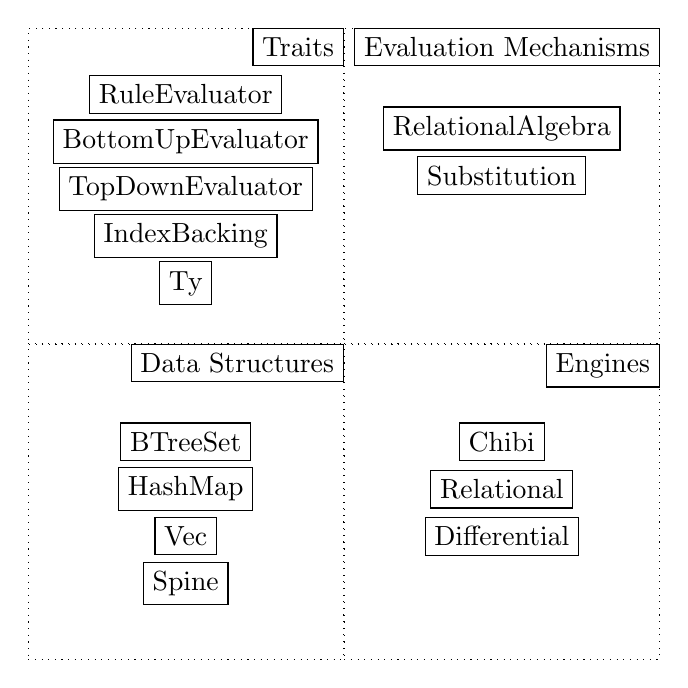
\begin{tikzpicture}[node distance=6mm]
		\begin{scope}
			\node (traits) at (0, 0) [draw, dotted, rectangle, minimum width=4cm, minimum height=4cm] {};
			\node (traits_title) at (traits.north east) [draw, anchor = north east] {Traits};

			\node (ev_mec) at (traits.east) [draw, dotted, rectangle, minimum width=4cm, minimum height=4cm, anchor=west] {};
			\node (ev_mec_title) at (ev_mec.north east) [draw, anchor=north east] {Evaluation Mechanisms};

			\node (ds) at (traits.south) [draw, dotted, rectangle, minimum width=4cm, minimum height=4cm, anchor=north] {};
			\node (ds_title) at (ds.north east) [draw, anchor=north east] {Data Structures};

			\node (engines) at (ds.east) [draw, dotted, rectangle, minimum width=4cm, minimum height=4cm, anchor=west] {};
			\node (engines_title) at (engines.north east) [draw, anchor=north east] {Engines};
		\end{scope}

		% Traits
		\begin{scope}
			\node (insta) [draw, below = 6mm of traits.north] {RuleEvaluator};
			\node (bupe) [draw, below of = insta] {BottomUpEvaluator};
			\node (tode) at (traits) [draw, below of = bupe] {TopDownEvaluator};
			\node (idx) at (traits) [draw, below of = tode] {IndexBacking};
			\node (ty) at (traits.south) [draw, below of = idx] {Ty};
		\end{scope}

		% Data Structures

		\begin{scope}
			\node (btset) [draw, below = 10mm of ds.north] {BTreeSet};
			\node (hashm) at (ds) [draw, below of = btset] {HashMap};
			\node (vecto) at (ds) [draw, below of = hashm] {Vec};
			\node (spine) at (ds) [draw, below of = vecto] {Spine};
		\end{scope}

		% Evaluation Mechanisms

		\begin{scope}
			\node (relal) [draw, below = 10mm of ev_mec.north] {RelationalAlgebra};
			\node (subst) at (ds) [draw, below of = relal] {Substitution};
		\end{scope}

		% Engines

		\begin{scope}
			\node (chibi) [draw, below = 10mm of engines.north] {Chibi};
			\node (relational) at (engines) [draw, below of = chibi] {Relational};
			\node (differential) at (engines) [draw, below of = relational] {Differential};
		\end{scope}

	\end{tikzpicture}
	\caption{Shapiro Components}
	\label{fig:shapiro_comp}
\end{figure}

\section{System}

In this section we provide a technical overview of the implemented reasoners, alongside a novel optimization
technique for the substitution-based method, that at the cost of slightly increased memory usage, avoids the
potential polynomial blowup, making the method suitable to be used with DRED, furthermore, we then port it to
differential dataflow

\subsection{Chibi}

\subsection{Relational}

\subsection{Differential}

\section{Benchmarks}

The aim of the experiments is to showcase relative performance, and scalability. Given that all reasoners to be compared share as much code as possible, are written in the same
programming language, and use the same elementary memory model, possibly strong empirical statements can be made with respect to the specificities of their implementation.

\textbf{Setup.} The experiments were run on commodity hardware, a MacbookPro with an M1 Pro processor and 16GB of ram, and in no test did swap memory was reached for.
Rust version 1.65 was used.

\begin{table}[]
	\begin{tabular}{llll}
		Dataset    & Area             & Programs   \\
		linux      & program analysis & CSPA, CSDA \\
		postgresql & program analysis & CSPA, CSDA \\
		httpd      & program analysis & CSPA, CSDA \\
		LUBM       & semantic web     & RhoDFS
	\end{tabular}
	\label{table:datasets}
\end{table}

\textbf{Datasets.} On table \ref{table:datasets} all datasets and program names, or acronyms, are shown. There are two areas of interest. The first is program analysis, a highly active research
field that has propelled significant advancements in datalog reasoners, such as \cite{incA}, an incremental datalog engine extended with lattices and recursive aggregates, and
souffle\cite{souffle}, a priceless source of more than half a dozen papers on the engineering aspects of a reasoner. While the latter's point is to run pre-defined programs over
large datasets, the former is meant for more dynamic scenarios, such as in running and maintaining program analyses.

The semantic web has very unique use-cases for datalog, and are the leading source of research in extending datalog. Seeking ways to introduce tuple-generating dependencies to
programs, with evaluation remaining tractable, has been one of the most active research directions, with highly-influential papers establishing new families of datalog
languages\cite{datalog_plus_minus} and thoroughly exploring their complexity classes alongside further expansions\cite{sticky,warded,monadic}.

These advancements have been somewhat tested in practice, albeit with no full reference implementation having been specified. The most comprehensive, and recent, is closed-source\cite{vadalog}.
The leading datalog engine in general, is also closed-source\cite{rdfox}, and is tailored specifically to the semantic web.

\begin{exmp}{Context-sensitive Points-to Analysis Program}
	\tiny
	\begin{align}
		valueFlow(?x, ?y) \leftarrow assign(?x, ?y)                                                 \\
		valueFlow(?x, ?z) \leftarrow assign(?x, ?y), memoryAlias(?y, ?z)                            \\
		valueFlow(?x, ?z) \leftarrow valueFlow(?x, ?y), valueFlow(?y, ?z)                           \\
		memoryAlias(?x, ?w) \leftarrow dereference(?x, ?y), valueAlias(?y, ?z), dereference(?z, ?w) \\
		valueAlias(?y, ?z) \leftarrow valueFlow(?x, ?y), valueFlow(?x, ?z)                          \\
		valueAlias(?y, ?z) \leftarrow valueFlow(?x, ?y), memoryAlias(?x, ?w), valueFlow(?w, ?z)     \\
		valueFlow(?x, ?x) \leftarrow assign(?x, ?y)                                                 \\
		valueFlow(?x, ?x) \leftarrow assign(?y, ?x)                                                 \\
		memoryAlias(?x, ?x) \leftarrow assign(?y, ?x)                                               \\
		memoryAlias(?x, ?x) \leftarrow assign(?x, ?y)
	\end{align}
	\label{program:cspa}
\end{exmp}

\begin{exmp}{Context-sensitive Dataflow Analysis}
	\tiny
	\begin{align}
		null(?x, ?y) \leftarrow nullEdge(?x, ?y) \\
		null(?x, ?y) \leftarrow null(?x, ?y), arc(?y, ?z)
	\end{align}
	\label{program:csda}
\end{exmp}

\begin{exmp}{RhoDFS inference rules}
	\tiny
	\begin{align}
		A(?y, rdf:type, ?x) \leftarrow T(?a, rdfs:domain, ?x), A(?y, ?a, ?z)                                  \\
		A(?z, rdf:type, ?x) \leftarrow T(?a, rdfs:range, ?x), A(?y, ?a, ?z)                                   \\
		T(?x, rdfs:subPropertyOf, ?z) \leftarrow T(?x, rdfs:subPropertyOf, ?y), T(?y, rdfs:subPropertyOf, ?z) \\
		T(?x, rdfs:subClassOf, ?z) \leftarrow T(?x, rdfs:subClassOf, ?y), T(?y, rdfs:subClassOf, ?z)          \\
		A(?z, rdf:type, ?y) \leftarrow T(?x, rdfs:subClassOf, ?y), A(?z, rdf:type, ?x)                        \\
		A(?x, ?b, ?y) \leftarrow T(?a, rdfs:subPropertyOf, ?b), A(?x, ?a, ?y)
	\end{align}
	\label{program:rhodfs}
\end{exmp}

The first program, \ref{program:cspa}\cite{graspan}, expresses pointer analysis, whose goal is to establish which assignments yield value aliases and memory aliases as a reachability problem. Program \ref{program:csda} directly models checking a program's control-flow graph for null edges as a simple transitive-closure computation. The last program, \ref{program:rhodfs}, is used to materialize the non-trivial inference rules from RDFS\cite{rdfs}, a popular data modelling logic for adding semantics to RDF\cite{rdf} data.

\subsection{COST}

\begin{figure}[htb!]
	\centering
	\includegraphics[width=.45\textwidth,height=\textheight,keepaspectratio]{COST}
	\caption{The COST of differential reasoner}
	\label{benchmark:cost}
\end{figure}

Benchmark \cite{benchmark:cost} seeks to answer an important question that is often overlooked, what is the configuration that outperforms a single thread(COST)? this can be convincingly answered in shapiro. As it can be seen, on the LUBM dataset, a synthetic infinitely-scalable ontology, in order to fully materialize all data at once, differential reasoner performs on par with the substitution-based reasoner, showcasing the very little overhead that differential dataflow has, given that it implements the same algorithm as the substitution-based reasoner.

\subsection{Scalability.}

\begin{figure}[htb!]
	\centering
	\subfloat[]{\includegraphics[width=.5\textwidth,height=\textheight,keepaspectratio]{addition}\label{benchmark:scalability_addition}}%
	\subfloat[]{\includegraphics[width=.5\textwidth,height=\textheight,keepaspectratio]{deletion}\label{benchmark:scalability_deletion}}\\
	\caption{Scalability with respect to update size}
	\label{benchmark:scalability}
\end{figure}

Scalability is measured over the LUBM dataset over increasingly larger relative updates. There are two kinds of updates: additions and deletions, both as a percentage of the total data. It is evident from benchmark \cite{benchmark:scalability} that all reasoners scale linearly with respect to the increasing amount of data, however, there is a significant difference with respect to updates. Both non-differential reasoners seem to get polynomially slower with bigger deletion update sizes than differential dataflow.

\subsection{Multiple Datasets.}

\begin{figure}[ht]
	\centering
	\subfloat[]{\includegraphics[width=.5\textwidth,height=\textheight,keepaspectratio]{CSDA}\label{benchmark:CSDA}}%
	\subfloat[]{\includegraphics[width=.5\textwidth,height=\textheight,keepaspectratio]{CSPA}\label{benchmark:CSPA}}\\
	\caption{Multiple programs with different datasets}
	\label{benchmark:scalability}
\end{figure}

The last benchmark, pertaining to program analysis, is used to explore the possibly performance differences for completely different datasets, with the same programs. Benchmark \cite{benchmark:csda} is the most surprising, since differential dataflow significantly outperforms the other implementations, while this isn't the case in any other benchmark. The rationale behind that, is that in both non-differential reasoners, iteration implies cloning a non-trivial amount of data, therefore generating a large amount of allocations, while the differential version also makes a large number of allocations, it parallelizes iterations, due to its partially-ordered timestamp, being able to concurrently progress multiple independent transitive chains at once.

\section{Conclusion}

In this paper we introduced Shapiro, a reasoning framework whose core value proposition is in providing modular components to build datalog reasoners. We utilized it to build a reasoner with a promising differential computation framework, differential dataflow, and evaluated it against two other reference implementations. The differential implementation bested its non-differential counterpart, showing very little overhead, however, it did not get close to a relational implementation, the current state-of-the-art approach, nor could it scale as well as the others, nonetheless, it did manage to handle updates in a much more efficient manner, performing exactly as well in additions as in deletions, therefore being much more efficient in practical situations, where no assumption about the kind of update can be made, than both implementations. This yields promising evidence as to the suitability of differential dataflow's computational model to datalog evaluation.
%
%
% \textbf{Contributions.} In this article we make several contributions to clarifying, benchmarking
% and easing pushing the boundaries of datalog evaluation engineering research further by
% providing performant and open-source implementations of single-threaded, parallel and distributed evaluators.
%
% \begin{itemize}
%   \item \textbf{Techniques and Guidelines.} We study the challenge of building a reasoner from scratch,
%         with no underlying framework, and ponder over all decisions necessary in order to bring that to fruition,
%         alongside with relevant recent literature.
%   \item \textbf{Differential Dataflow.} We accurately investigate the suitability of differential
%         dataflow for datalog, and showcase how does it fare against the ubiquitous DRED and semi-naive
%         evaluation based reasoners with the same language, base and with the same data format.
%   \item \textbf{Framework.} All code outputs of this article are coalesced in a rust library named shapiro,
%         consisted of a datalog to relational algebra rewriter, a relational algebra evaluator, and two datalog engines,
%         one that is parallel-capable and supports both substitution-based and relational algebra methods, and other that
%         relies on the state-of-the-art differential dataflow\cite{differential_dataflow} distribution computation framework.
%         The main expected outcome of this library is to provide well understood and reasoned about baseline implementations
%         from where future research can take advantage of, and reliable COST configurations can be attained.
%   \item \textbf{Benchmarking.} We perform two thorough benchmark suites. One evaluates the performance of the developed
%         relational reasoner with multiple different index data structures and common optimizations, such as string interning
%         and simple parallelism, and another that attempts to attain the COST of the reasoner built on top of differential
%         dataflow. The selected datasets are either from the program analysis, heavy users of not-distributed datalog, or from
%         the semantic web community, which has multiple popular infinitely-scalable benchmarks.
% \end{itemize}

\bibliographystyle{ACM-Reference-Format}
\bibliography{software}

\end{document}
\endinput
%%% Local Variables:
%%% mode: latex
%%% TeX-master: t
%%% End:
